


\documentclass[11pt]{amsart}

\usepackage{fancyhdr}
\usepackage{amsmath, amscd}
\usepackage{enumerate}
\usepackage{amsthm}
\usepackage{amssymb}
\usepackage[pdftex]{graphicx}
\usepackage{verbatim}
\usepackage[all]{xy}
\usepackage{booktabs}
%\usepackage{hyperref}
%\usepackage{homework}
%\usepackage[top=1.5in, bottom=1in, left=1.25in, right=1.25in]{geometry}

\input{gsDefns}


\begin{document}

\title[Finding the best box to pack an order into]{Finding the best box to pack an order into}
\date{\today}
\author{Gautam Sisodia}
\maketitle

\section*{Introduction}

\subsection*{The problem}

Given a customer order and a set of boxes, what's the optimal box to pack the order into? The customer order is a list of products with dimensions.

My naming convention for the faces of the box is shown below.

\begin{figure}[h]
%\centering
\makebox[0.8\textwidth][c]{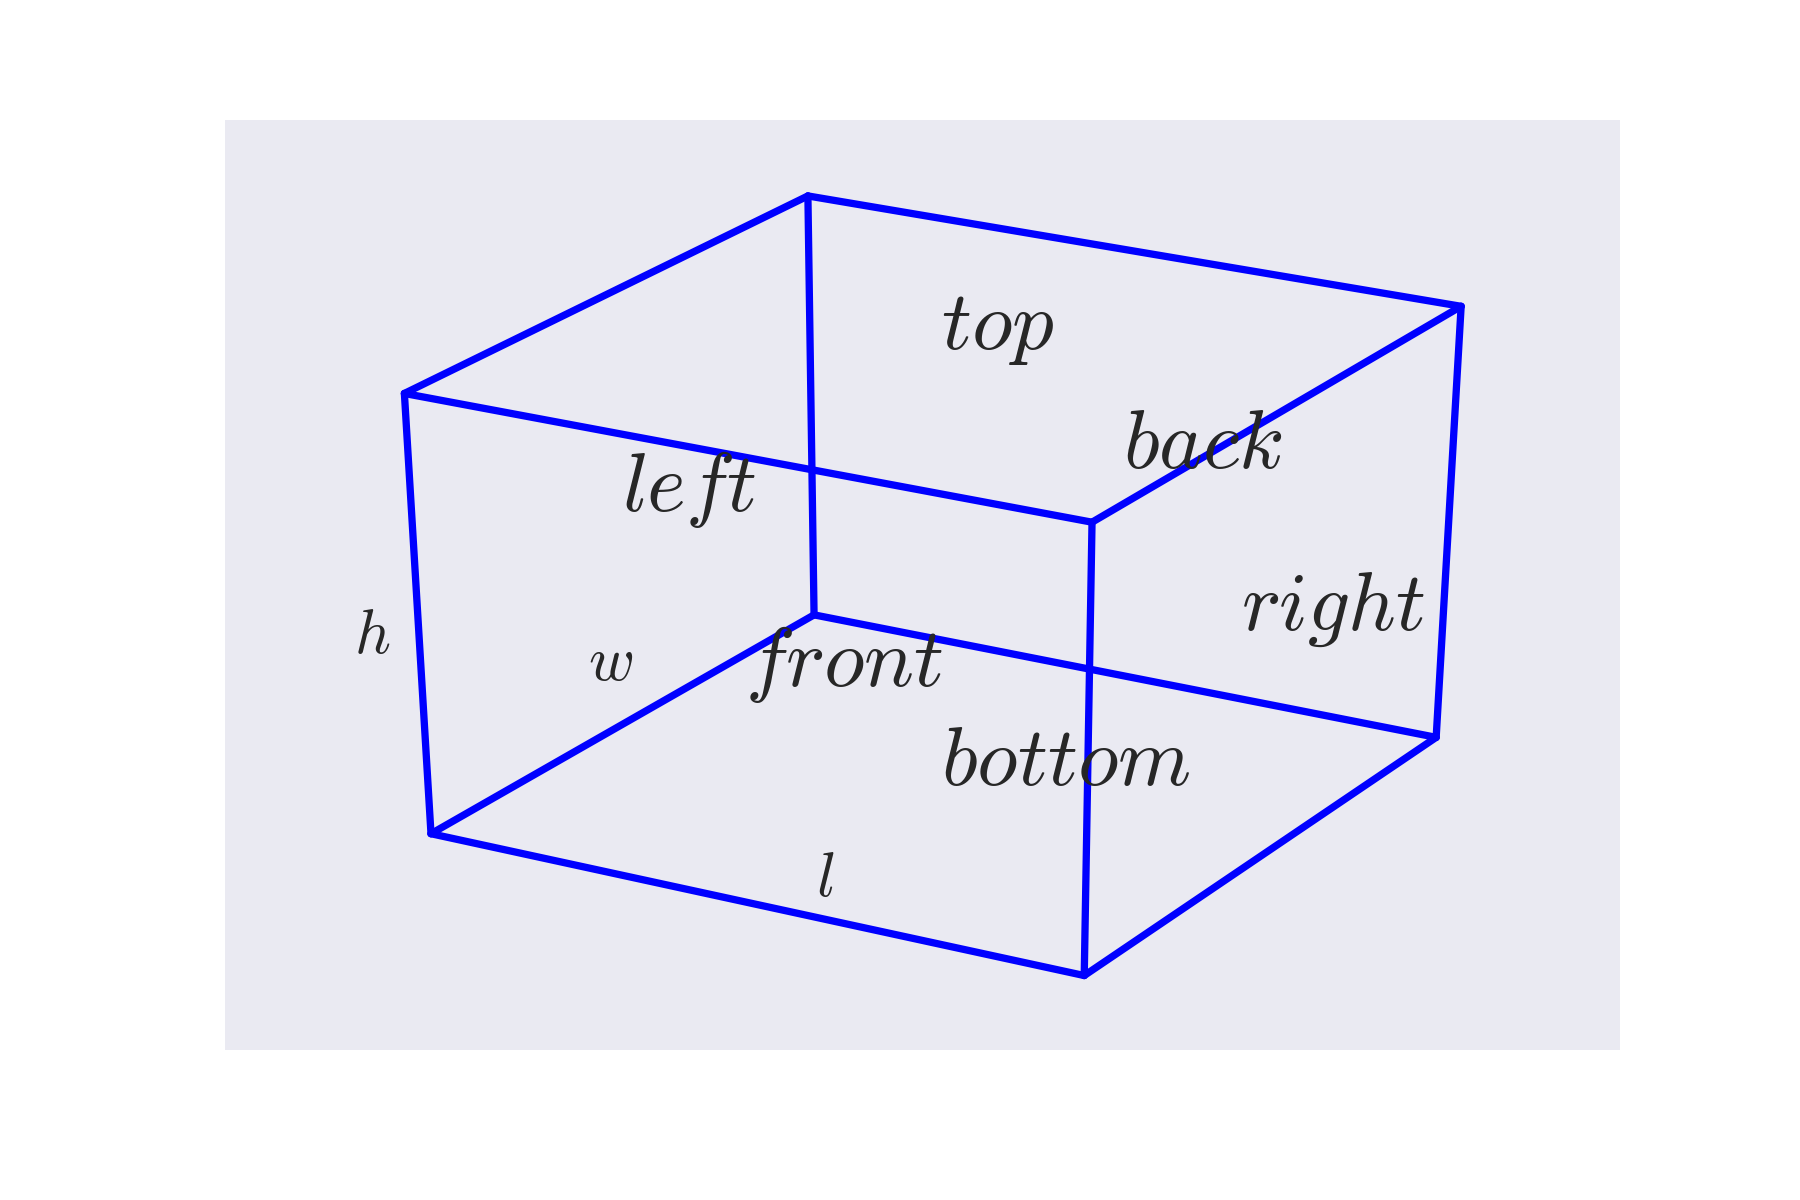
\includegraphics[width = 0.8\textwidth]{box}}
\label{apmd}
\end{figure}

I assume that the orientation of each product in the box is fixed so that the faces of the products line up with the corresponding faces of the box.

\subsection*{What do we mean by optimal?}

I take optimal to mean smallest surface area. I chose surface area over other metrics like volume for two reasons: the cost of a box is proportional to its surface area, and in terms of ease of transportation and delivery, cube-shaped boxes are easier to handle than long and wide ones.

\section*{The algorithm}

\subsection*{A description}

My algorithm for finding the optimal box first orders the boxes by surface area and steps through the boxes from smallest to largest. For each box, we try to pack the products into the box. If we can, we return that box as the optimal choice. If not, we move on to the next largest box.

To determine if the products can be packed into a given box, we first make sure the volume of the box is at least the total volume of the products, and in each dimension the box is at least as large as the largest product in that dimension. If the box passes these simple checks, then we try to construct a packing.

We pack the products in order from largest surface area to smallest. We start by putting the largest product in the left front bottom (lfb) corner. For the sake of space efficiency, we want to place products adjacent to each other, so for each product, we go through the possible coordinates of its lfb corner, checking to see if the product fits in that space. If it does, we place it there, update the list of possible coordinates, and move to the next product.

We keep track of the position of each packed product by recording the coordinates of its left front bottom (l.f.b.) corner (taking the l.f.b.\ corner of the box to be the origin).

\subsection*{Pseudo code}

\begin{figure}[h]
%\centering
\makebox[0.8\textwidth][c]{\includegraphics[width = 0.8\textwidth]{pic2_391_179_3}}
\label{apmd}
\end{figure}

\subsection*{An example}

\subsection*{Advantages and disadvantages}

ad
*adapt to different optimal metrics

dis
*orientation

\section*{Dividing a big order into multiple boxes}

\end{document}
